\input{configuration}

\title{Lecture 25 --- Load Testing}

\author{Jeff Zarnett\\ \small \texttt{jzarnett@uwaterloo.ca}}
\institute{Department of Electrical and Computer Engineering \\
  University of Waterloo}
\date{\today}


\begin{document}

\begin{frame}
  \titlepage

\end{frame}

\begin{frame}
\frametitle{From Observation to Load Testing}

We talked about observability, but we want to also talk about scalability.

Goal: scale number of users,

\[ 1 \rightarrow 100 \rightarrow 10 000 000. \]


\begin{center}
	\includegraphics[width=0.2\textwidth]{images/Rebel_Yell.jpg}\\
	\hfill ``In the midnight hour, she cries 'more, more, more''' - Billy Idol
\end{center}

\end{frame}


\begin{frame}
\frametitle{Not Hypothetical}

CFO: Can this system handle $10\times$ as many users as we have now?

My answer has to have numbers. Analysis and \alert{load testing}.

\begin{center}
  
\includegraphics[width=0.4\textwidth]{images/loadbearing.jpg}
\end{center}

\end{frame}

\begin{frame}
\frametitle{Start With Why}
Why are we doing this?

\begin{itemize}
	\item A new system is being developed -- limits \& risks
	\item Workload increase; can we handle it?
	\item A sudden spike in workload is expected
	\item Uptime requirements: 99.99\%
	\item Plan has checkbox ``performance testing''
\end{itemize}



\end{frame}

\begin{frame}
\frametitle{Reasons Why}

Each implies a slightly different kind of testing.

\begin{itemize}
	\item New system: average workload (plus buffer)
	\item Workload: what's our bottleneck?
	\item Spike: how to simulate it?
	\item Uptime: endurance!
\end{itemize}

(We'll ignore the last reason)

\end{frame}

\begin{frame}
\frametitle{Stress Test?}

Load testing is not the same as \alert{stress testing}.

\begin{center}
  
\includegraphics[width=0.5\textwidth]{images/barrescue.jpg}
\end{center}

We're not going into it, but you can apply load testing strategies turned up to the max to get stress test results.

\end{frame}

\begin{frame}
\frametitle{Making the Plan}

Let's make a test plan! Need answers to textit{who, what, where, when, \& why}.

We already covered why and that tells us about what.

Who? We will!

When? Now!

\end{frame}

\begin{frame}
\frametitle{Plan Signoff}

How detailed the plan needs to be is going to depend on your organization, and the same applies for how many sign-offs (if any!) you need on the plan. 

\begin{center}
  
\includegraphics[width=0.5\textwidth]{images/signoff.jpg}
\end{center}

... let's not get sidetracked.

\end{frame}


\begin{frame}
\frametitle{What Do We Need?}

\textit{What} will be tested?


\textit{How} will it be tested?


\textit{How do we know} if the test is passed?

\end{frame}

\begin{frame}
\frametitle{What Workflows To Test}

We cannot test everything; cost \& effort are too high.

Do we already know what the rate-limiting steps are?

Maybe need to add observability first to identify those.

\begin{center}
  
\includegraphics[width=0.4\textwidth]{images/badtime.jpg}
\end{center}

\end{frame}

\begin{frame}
\frametitle{Excuse Me, I'm New Here}

What if it's a new system?

Critical is determined by product requirements:\\
\begin{itemize}
	\item Computationally intensive work?
	\item User experience?
	\item External timing requirements?
\end{itemize}

\end{frame}

\begin{frame}
\frametitle{Other Load Scenarios}

If utilization is low it might not be clear what the bottlenecks are.\\
\quad Might need to guess and revise those later.

\begin{center}
  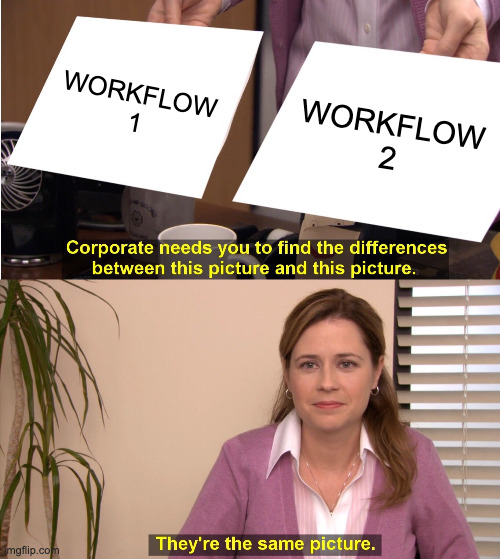
\includegraphics[width=0.4\textwidth]{images/workflow.jpg}
\end{center}

If it's uptime requirements, we need endurance tests.\\
\quad We'll come back to those.

\end{frame}

\begin{frame}
\frametitle{How to Test Them}
Might need to provision additional (virtual) hardware.

Regular testing tools might not be correct; may need a script.

Dev and production aren't the same, but how do they differ?

\end{frame}

\begin{frame}
\frametitle{Maybe Don't Do This}

\begin{center}
	\includegraphics[width=0.4\textwidth]{images/testinprod.png}
\end{center}

... Not quite what I mean.

\end{frame}

\begin{frame}
\frametitle{Hardware Principle}



Scalability testing $\neq$  QA testing.

Dev + QA on local computer.\\
\quad Your concerns: Is it right? Is it fast enough?

Fine, but it's no way to test if it scales. 


\end{frame}



\begin{frame}
\frametitle{Hardware Principle}



Test on prod-like machines: low-end systems have very different limiting factors.

Your laptop: limited by 16GB of RAM.\\
Prod server: 128GB of RAM.


So you might spend a great deal of time worrying about RAM usage and it just doesn't matter.


\end{frame}



\begin{frame}
\frametitle{Reality Principle}

\begin{center}
	\includegraphics[width=0.5\textwidth]{images/qa.png}
\end{center}


\end{frame}


\begin{frame}
\frametitle{Reality Principle}


Use a ``real'' workload.\\
\quad Maybe not actual live customer data, but try to come close.

Limited test data/scenarios $\Rightarrow$ inaccurate test results.


Your tests run summary reports occasionally\ldots\\
\quad your users might run them every hour. 

\end{frame}



\begin{frame}
\frametitle{Volume Principle}


``More is the new more.'' 

Lighter workloads OK for regression testing. 

To see how your system performs under pressure, you actually need to put it under pressure. 

Can simulate pressure by limiting RAM or running something very CPU-intensive concurrently, but it's just not the same.

\end{frame}



\begin{frame}
\frametitle{Reproducibility and Regression Testing}

Science rule 1: results need to be reproducible!


There is likely some variance in runs during load testing due to the natural randomness of the OS, scheduler, luck, etc.


\end{frame}


\begin{frame}
\frametitle{Endurance Tests -- How Long?}

You're familiar with the idea that endurance is different from peak workload.

\begin{center}
  
\includegraphics[width=0.4\textwidth]{images/running-worse.jpg}
\end{center}

\end{frame}

\begin{frame}
\frametitle{Let's Go For A Run}

Can I [JZ] run at 10 km/h for...\\
\begin{itemize}
	\item 1 minute? Yes, of course!
	\item 30 minutes (5 km)? Yes!
	\item 60 minutes (10 km)? Yes (with difficulty).
	\item 4 hours (40 km)? No.
\end{itemize}

But if we just observed my running for 15 minutes, we might conclude I could run at 10 km/h indefinitely, but that's not true.

\end{frame}

\begin{frame}
\frametitle{Cumulative Negative Effects}

\begin{center}
  
\includegraphics[width=0.7\textwidth]{images/tetris.jpg}
\end{center}

If our sample period is 15 minutes, it's not long enough to reflect the cumulative negative effects that contribute to my slowing down and being forced to stop. 

\end{frame}

\begin{frame}
\frametitle{Wait, CPUs Don't Get Tired}

\begin{center}
  
\includegraphics[width=0.5\textwidth]{images/dont-get-tired.jpg}
\end{center}

Their parts accumulate fatigue, but not at the rate of a runner's muscles.

Yes, it's still a valid analogy. Consider a program that has a data hoarding issue.

\end{frame}

\begin{frame}
\frametitle{It'll Fit}

One outcome: \texttt{java.lang.OutOfMemoryError: Java heap space}

Same for filling up disk, exhausting file handles, log length.

Another example: holiday code freeze as unintentional endurance test.

\end{frame}

\begin{frame}
\frametitle{Okay, But How Long?}
Is 30 minutes of running the right amount? 3 hours?

Maybe it's product requirements again: e-commerce on Black Friday?

What about the maintenance window?

No easy answers.

\end{frame}


\begin{frame}
\frametitle{Evaluating Success}

\end{frame}

\end{document}